\makesection{Benchmarking}

\begin{frame}{Dataset - LFM\_1b\_artist}
\footnotesize
\begin{table}[H]
\centering
\begin{tabular}{|c|c|}
\hline
\textbf{Feature} & \textbf{Valore} \\
\hline
Numero di utenti & 120322 \\
\hline
Numero di item & 3123496 \\
\hline
Numero di interazioni & 65133026 \\
\hline
Sparsità & 0.9998266933373666 \\
\hline
avg\_interactions & 541.3226675088513 \\
\hline
\end{tabular}
\caption{Statistiche dataset LFM\_1b\_artist}
\end{table}

    Questo risultava essere troppo grande per le risorse a disposizione, quindi così processato:
    \begin{itemize}
        \item  \textbf{Filtraggio}: rimossi item e utenti con meno di 5 interazioni
        \item  \textbf{Sampling}:sampling casuale di 50000 items e 20000 utenti
        \item \textbf{Stratificazione}: Per ogni utente : 75\% , 50\%, 25\%
    \end{itemize}
\end{frame}




\begin{frame}{Dataset - MovieLens10M}
\footnotesize
    \begin{table}[H]
    \centering
    \begin{tabular}{|c|c|}
    \hline
    \textbf{Feature} & \textbf{Valore} \\
    \hline
    Numero di utenti & 69878 \\
    \hline
    Numero di item & 10677 \\
    \hline
    Numero di interazioni & 10000054 \\
    \hline
    Sparsità & 0.9865966722939162 \\
    \hline
    avg\_interactions & 143.10732991785684 \\
    \hline
    \end{tabular}
    \caption{Statistiche MovieLens10M}
    \end{table}
        Anche questo risultava essere troppo grande per le risorse a disposizione, quindi così processato:
        \begin{itemize}
            \item  \textbf{Filtraggio}: rimossi item e utenti con meno di 5 interazioni
            \item  \textbf{Sampling}:sampling casuale di 50000 utenti e 10000 items
        \end{itemize}
    \end{frame}


\begin{frame}{Emissioni - Risultati}
    \begin{table}[H]
        \centering
        \footnotesize
        \setlength\tabcolsep{0pt}
        \begin{tabularx}{\textwidth}{|X|X|}
            \hline
            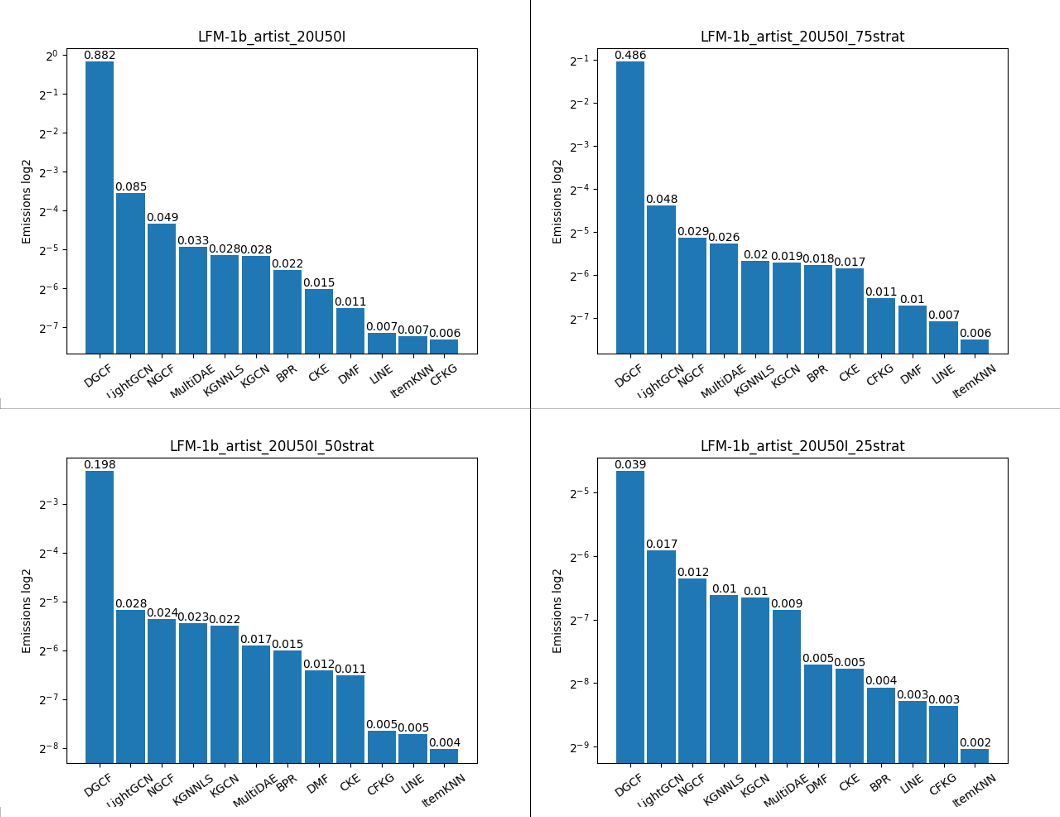
\includegraphics[width=\linewidth, trim=0 0 0 0]{images/EmissioniLFM.png} & 
            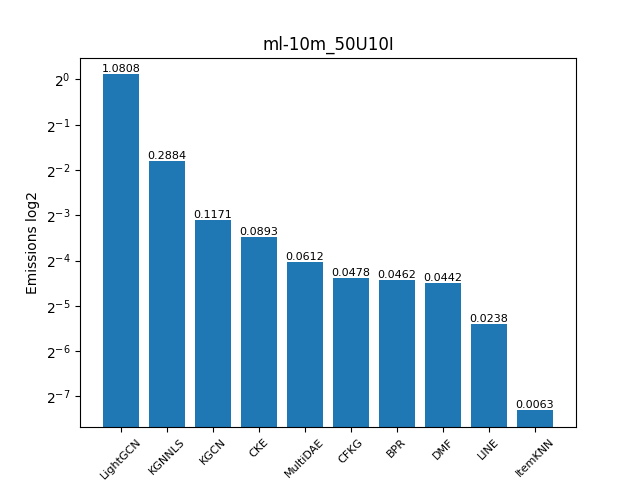
\includegraphics[width=\linewidth, trim=0 0 0 0]{images/emissions_ml-10m_50U10I.png} \\
            \hline
        \end{tabularx}
        \caption{Emissioni di CO2 per i vari modelli}
    \end{table}
\end{frame}


\begin{frame}{Trade - Off}
    \begin{figure}[H]
    \centering
    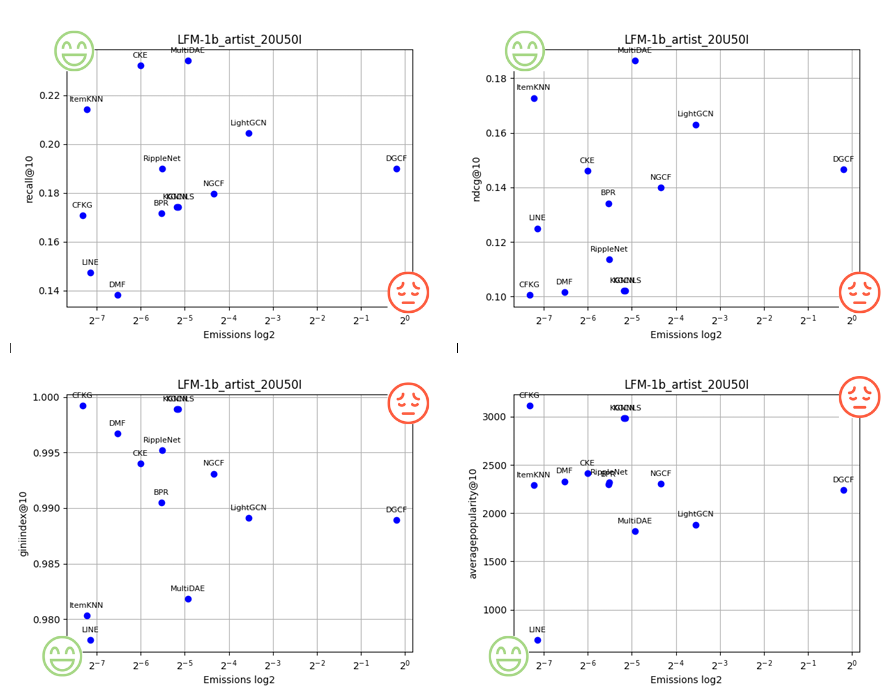
\includegraphics[height=0.7\textheight, width=0.7\textwidth]{images/TradeOff.png}
    \caption{Esempio di trade-off tra emissioni e performance}
\end{figure}
\end{frame}




\begin{frame}{Regressore - Dataset Completo}
    \begin{wrapfigure}{r}{0.5\textwidth}
    \centering
    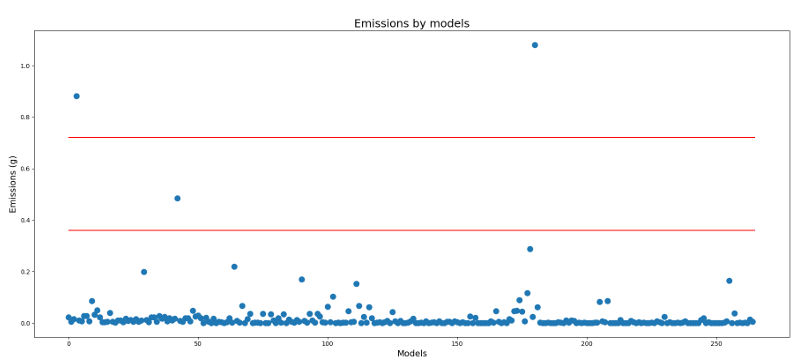
\includegraphics[width=0.5\textwidth]{images/distribuzioneCompleta.png}
    \caption{Nuova distribuzione dei dati}
\end{wrapfigure}

Come è possibile notare i nuovi esperimenti hanno portato a un'ulteriore sbilanciamento nel dataset, in quanto tutti gli esperimenti con DGCF e altri modelli svettano sui risultati degli altri modelli in emissioni.

\end{frame}


\begin{frame}{Regressore - Analisi dei risultati Dataset Completo}
    \begin{wrapfigure}{r}{0.5\textwidth}
    \centering
    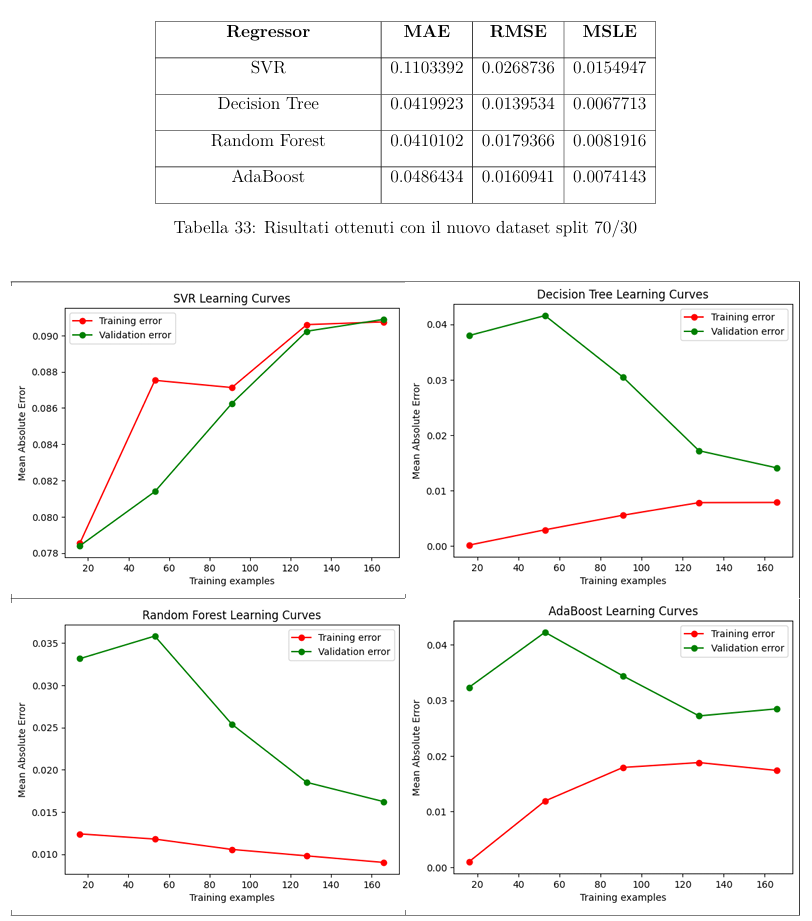
\includegraphics[width=0.3\textwidth]{images/RisultatiRegCompleto.png}
    \caption{Risultati con dataset completo}
\end{wrapfigure}
\small
Sono stati eseguti addestramenti con i seguenti split:
\begin{itemize}
    \item 50\% training, 50\% test
    \item 60\% training, 40\% test
    \item 70\% training, 30\% test
    \item 80\% training, 20\% test
    \item 90\% training, 10\% test
\end{itemize} 
I migliori risultati sono stati ottenuti con lo split 70-30, con il Decision Tree Regressor che risulta essere il modello migliore.
\end{frame}



\begin{frame}{Regressore - Dataset Azure}
    \begin{wrapfigure}{r}{0.5\textwidth}
    \centering
    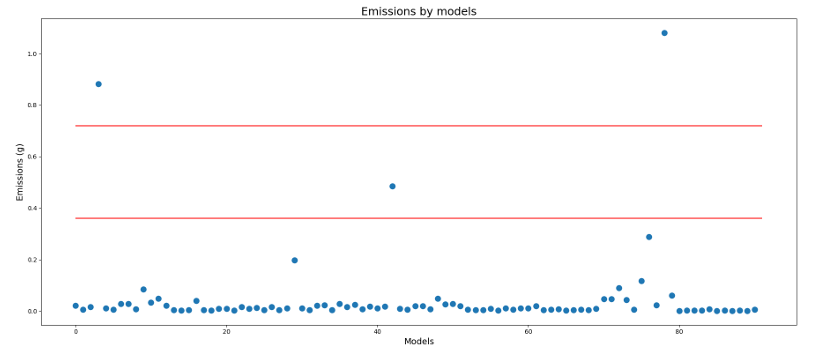
\includegraphics[width=0.5\textwidth]{images/distribuzioneAzure.png}
    \caption{Nuova distribuzione dei dati}
\end{wrapfigure}

E' stato creato un nuovo dataset con i risultati ottenuti solo sugli esperimenti eseguiti su Azure per avere un regressore specifico per gli esperimenti eseguiti su tale macchina.

\end{frame}


\begin{frame}{Regressore - Analisi dei risultati Dataset Azure}
    \begin{wrapfigure}{r}{0.5\textwidth}
    \centering
    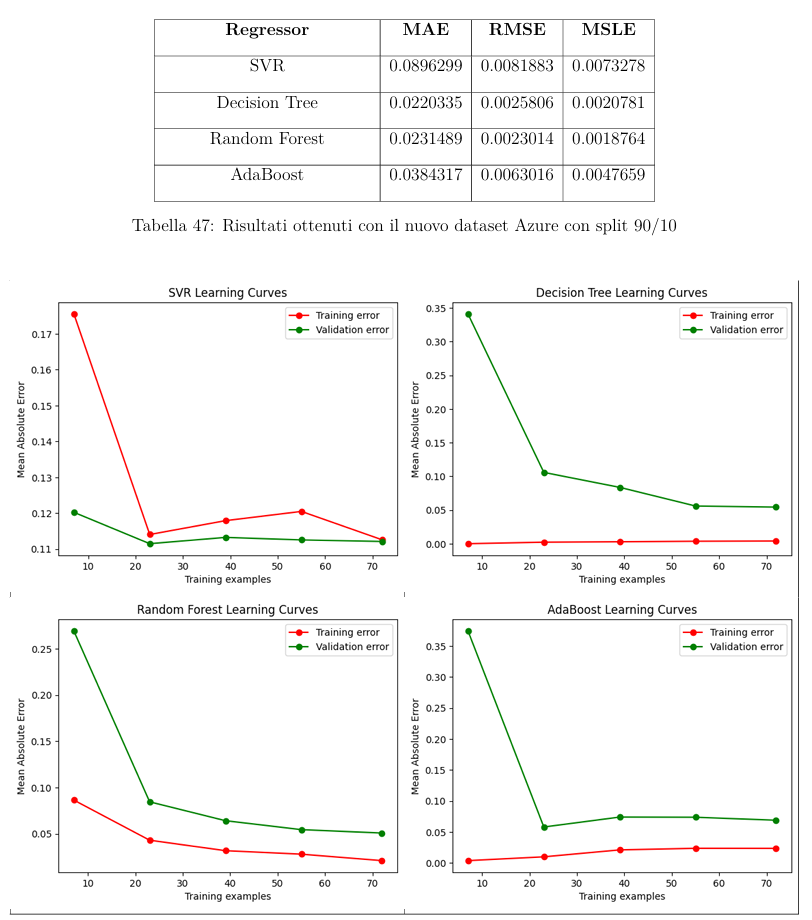
\includegraphics[width=0.3\textwidth]{images/RisultatiRegAzure.png}
    \caption{Risultati con dataset completo}
\end{wrapfigure}
\small
Sono stati eseguti addestramenti con i seguenti split:
\begin{itemize}
    \item 50\% training, 50\% test
    \item 60\% training, 40\% test
    \item 70\% training, 30\% test
    \item 80\% training, 20\% test
    \item 90\% training, 10\% test
\end{itemize} 
I migliori risultati sono stati ottenuti con lo split 90-10, con il Decision Tree Regressor che risulta essere il modello migliore.
\end{frame}


\begin{frame}{Errori nelle classi}
    \tiny 
Gli errori sono stati calcolati come segue:
\begin{itemize}
    \item \textbf{Errore assoluto}:\begin{equation*}
        |y - \hat{y}|
         \end{equation*}
    \item \textbf{Errore percentuale}: \begin{equation*}
        \frac{|y - \hat{y}|}{y} \cdot 100
    \end{equation*}
\end{itemize}

\textbf{Dataset Completo}

\begin{table}[H]
    \centering
    \begin{tabular}{|c|c|c|c|}
        \hline
        \textbf{Classe} &  \textbf{Numero elementi} & \textbf{Errore assoluto medio} & \textbf{Errore percentuale medio} \\ \hline
        low             & 78                & 0.021805                   & 813            \\ \hline
        medium          & 0                & -                  & -            \\ \hline
        high            & 2                & 0.790026                   & 80            \\ \hline
    \end{tabular}
    \caption{Errori delle classi per il dataset completo}
\end{table}

\textbf{Dataset Azure}

\begin{table}[H]
    \centering
    \begin{tabular}{|c|c|c|c|}
        \hline
        \textbf{Classe} &  \textbf{Numero elementi} & \textbf{Errore assoluto medio} & \textbf{Errore percentuale medio} \\ \hline
        low             & 78                & 0.044774                   & 188.63            \\ \hline
        medium          & 0                & -                  & -            \\ \hline
        high            & 2                & 0.588654                   & 66.76            \\ \hline
    \end{tabular}
    \caption{Errori delle classi per il dataset Azure}
\end{table}

\end{frame}